%!TEX root = ../Thesis.tex

\section{Trilateration}
Unlike triangulation, which uses the angles from known points, trilateration uses the distances from known points. This is the base concept behind GNSS. Satellite W sends out a radio signal at time X and it's position Y which the user received at time Z. The time difference is used to calculate the distance from the satellite's position, see Figure \ref{fig:trilateration}. With this information from multiple satellites, the users position is calculated. In reality, the distance from the satellite to the user has error in it, which will be explained in detail in Section \ref{sec:error sources}. The error alters the radius of the circle (or in 3D the sphere), see Figure \ref{fig:trilaterationtime}. The error is expressed as a clock bias, a change in time at the receiver side in order to find an intersection. As there are four variables to solve for, x, y, z and clock bias $b_u$, a minimum of four satellites are required to calculate the intersection. The range that has error in it is called the pseudorange.
\begin{figure}
\centering
\caption{Solve for Position using Trilateration}
\label{fig:trilateration}
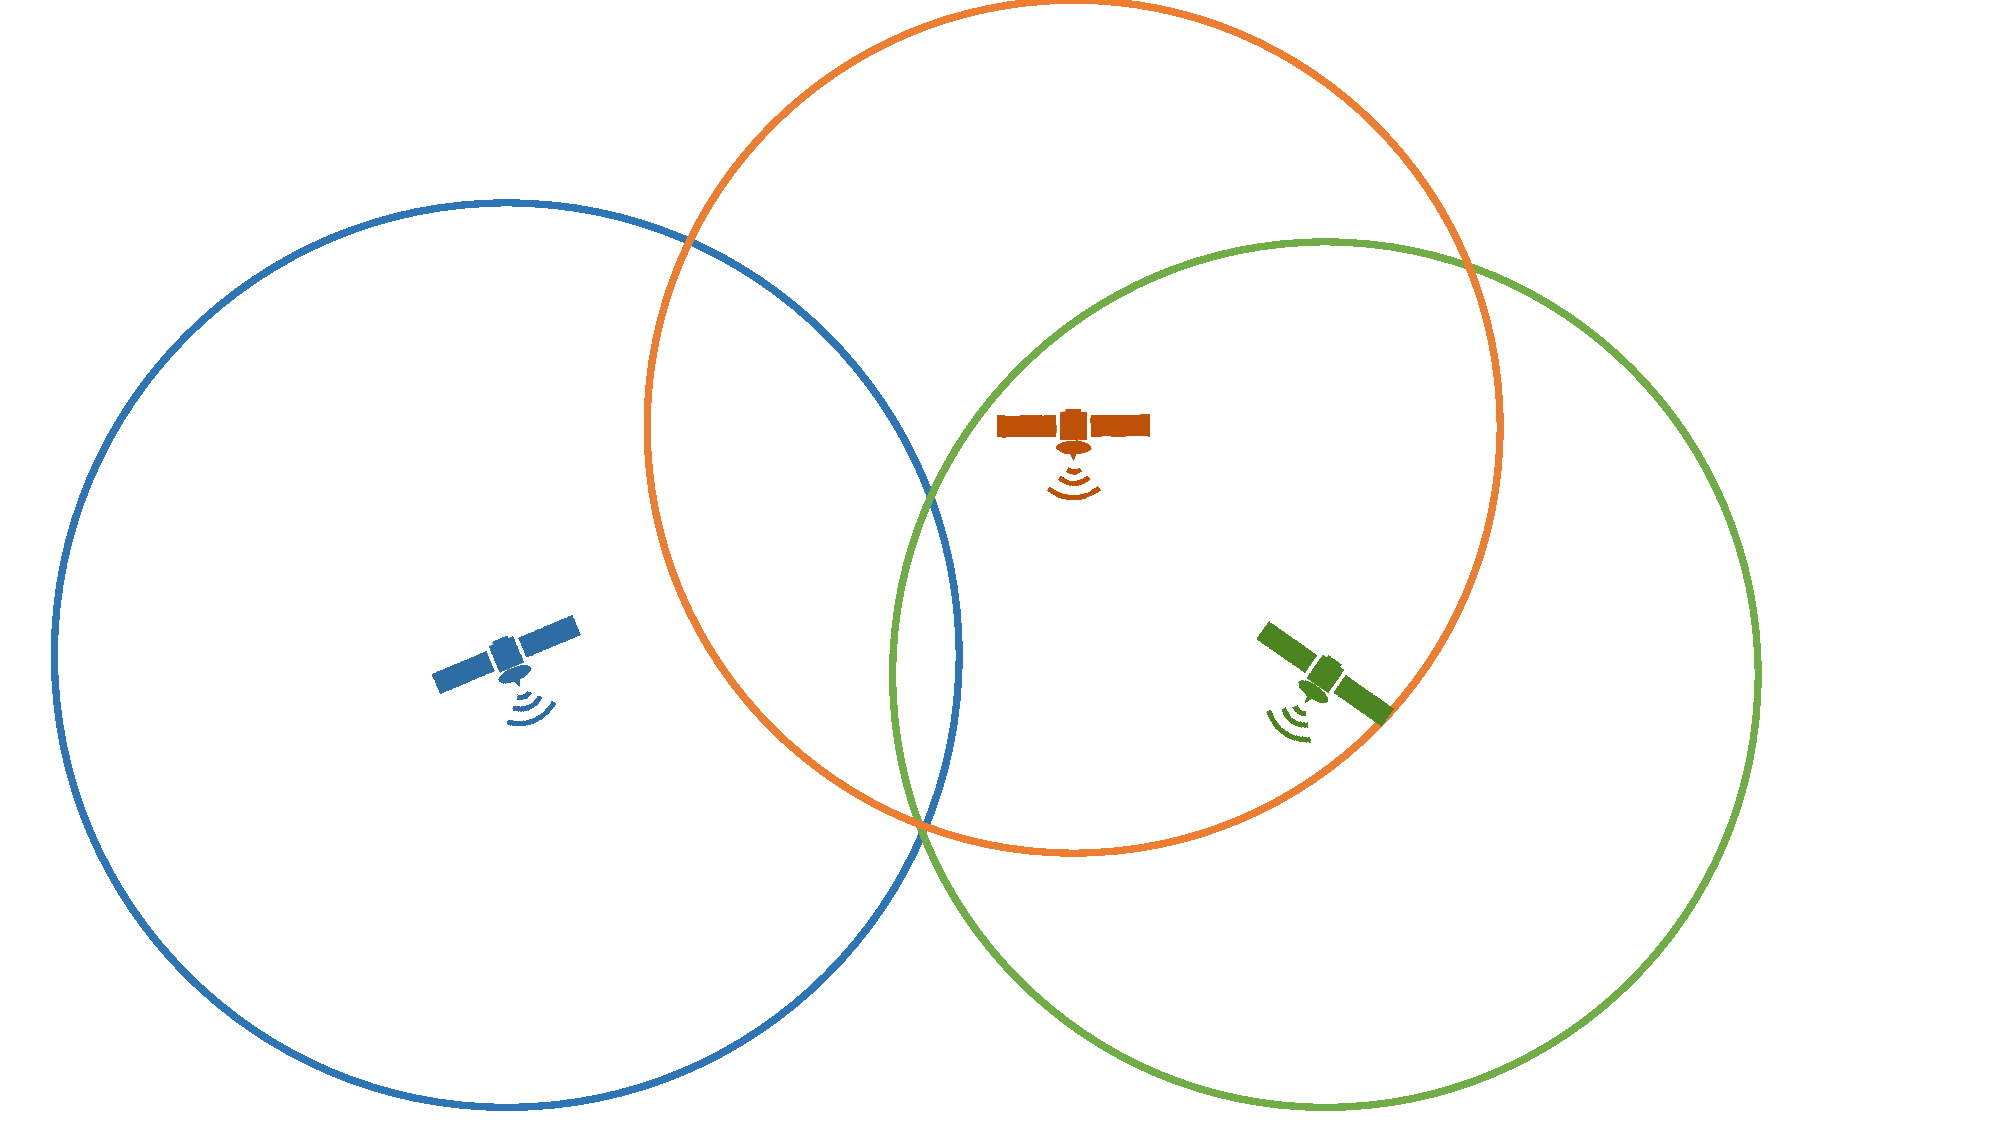
\includegraphics[width=0.7\linewidth]{ChapterLiteratureReview/trilateration}
\end{figure}
\begin{figure}
\centering
\caption{Solve for Position and Clock Bias using Trilateration}
\label{fig:trilaterationtime}
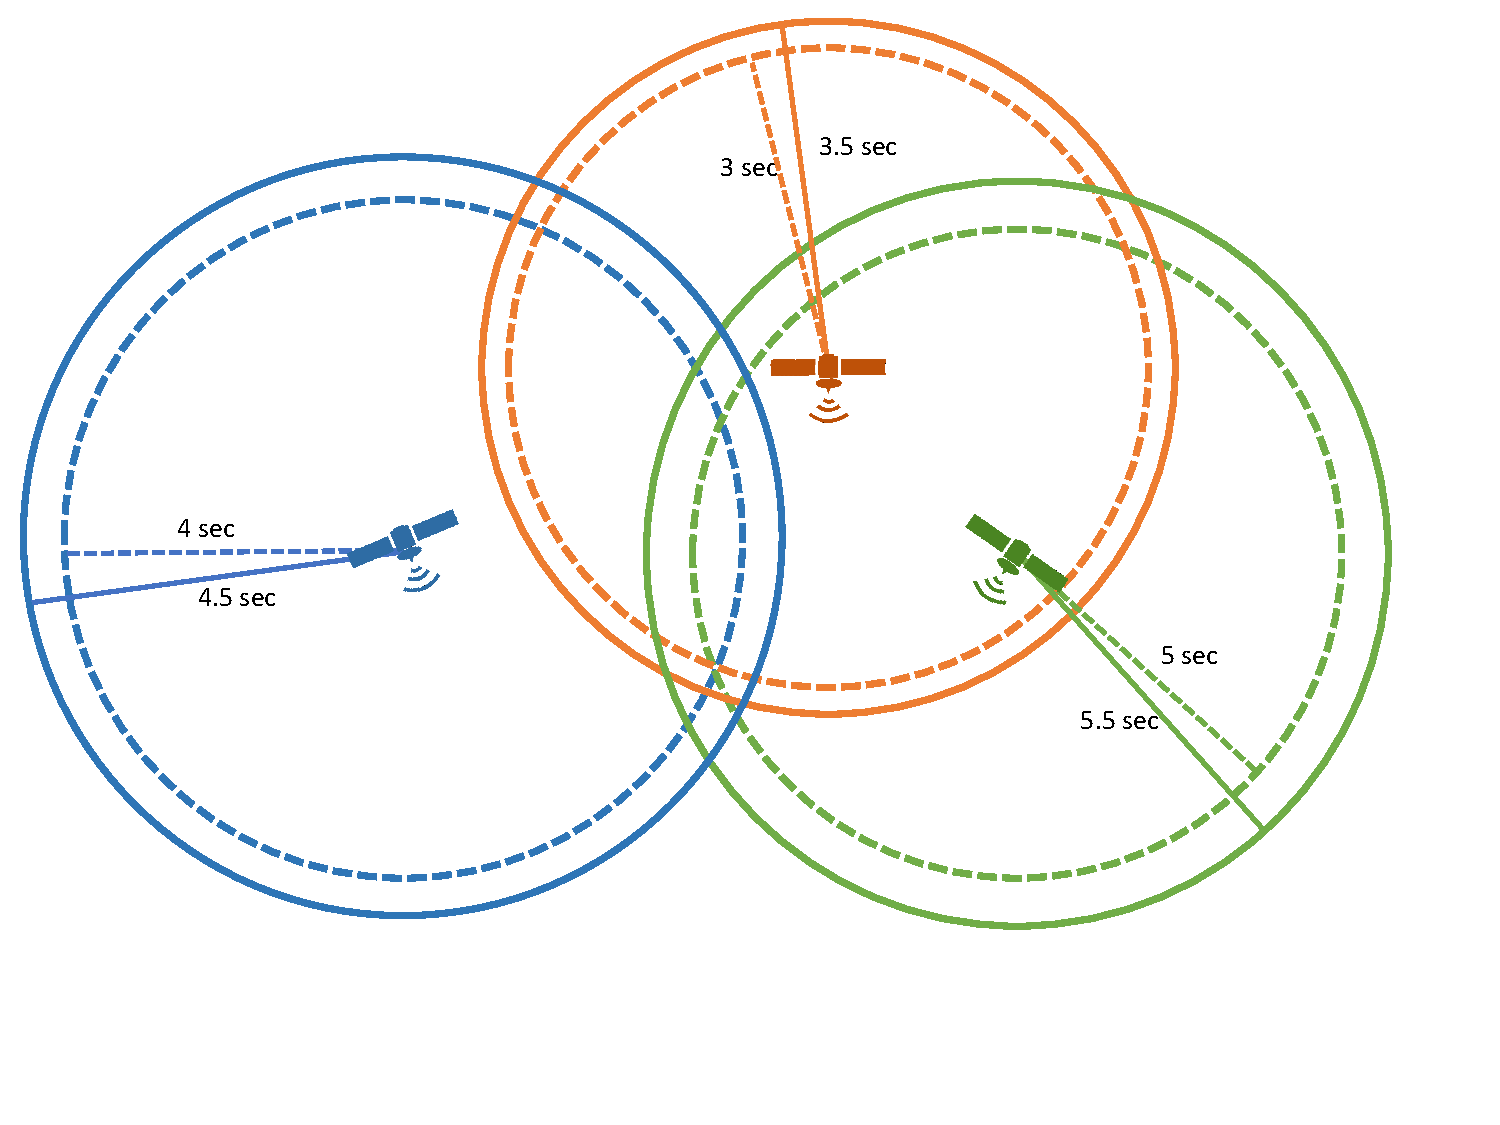
\includegraphics[width=0.7\linewidth]{ChapterLiteratureReview/trilaterationtime}
\end{figure}

\subsection{Nonlinear Least Squares} \label{sec:NLLS}
There may be more than four satellites in view, which creates an overdetermined system. There is not exact solution when the system has error, so it is solved via non-linear least squares (NLLS).
\begin{eqnarray}
\rho_i = \sqrt{(X_{SV_i}-x)^2+(Y_{SV_i}-y)^2+(Z_{SV_i}-z)^2} +cb_u + \epsilon
\end{eqnarray}
Where $\rho_i$ is the pseudorange of the receiver to satellite i, [$X_{SV_i},Y_{SV_i},Z_{SV_i}$] is the position of the satellite i, c is the speed of light, and $\epsilon$ is some measurement noise. NLLS is a standard algorithm that linearises about an estimate of the state variable
\begin{enumerate}
\item Assume an initial estimate of the system state
\item Linearise the system about the estimate by calculating the Jacobian
\item Calculate the residual between the estimated location and the measured ranges
\item Identify the residual due to the linearised system
\item Minimise the quadratic error to calculate the best linear step
\item Update the estimate using the linear step
\item Repeat until convergence
\end{enumerate}






- NLLS solve spheres

- ECEF frame of reference